\subsection{Model and training}\label{sec:model}

We focus on English-Dutch translation, for which we can ensure good command for both languages.
We train Transformer-base models \citep{vaswani2017attention} using Fairseq \citep{ott2019fairseq}.
Our training data consists of a collection of MT corpora bundled in \textsc{OPUS} \citep{tiedemann2020opus}, of which we use the English-Dutch subset provided by \citet{tiedemann-2020-tatoeba}, which contains 69M sentence pairs.\footnote{Visit \href{https://github.com/Helsinki-NLP/Tatoeba-Challenge/blob/master/data/README-v2020-07-28.md}{the Tatoeba challenge} for the \textsc{OPUS} training data.}
To examine the impact of the amount of training data -- a dimension that is relevant because compositionality is hypothesised to be more important when resources are scarcer -- we train one setup using the \textbf{full} dataset, one using $\frac{1}{8}$ of the data (\textbf{medium}), and one using one million source-target pairs in the \textbf{small} setup. 
For each setup, we train models with five seeds and average the results.

\begin{figure*}[!h]
    \centering
    \begin{subfigure}[b]{0.45\columnwidth}
        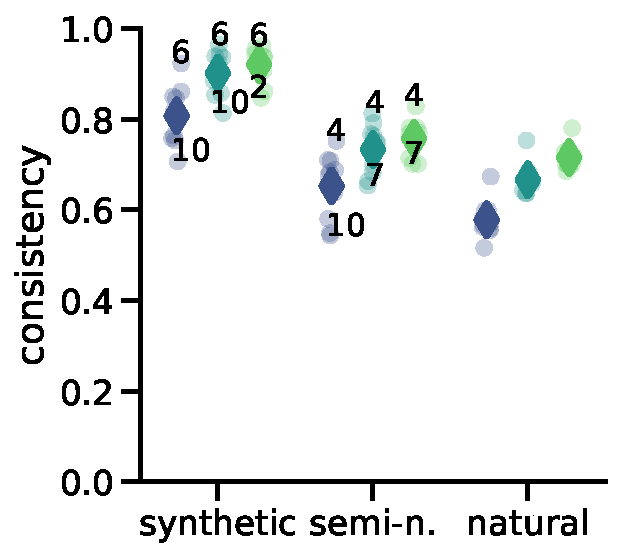
\includegraphics[width=\columnwidth]{figures/systematicity/s1p.pdf}
        \caption{$\text{S}_1 \rightarrow \text{S}_1^\prime$}
        \label{fig:systematicity_sconj_s1}
    \end{subfigure}
    \begin{subfigure}[b]{0.45\columnwidth}
        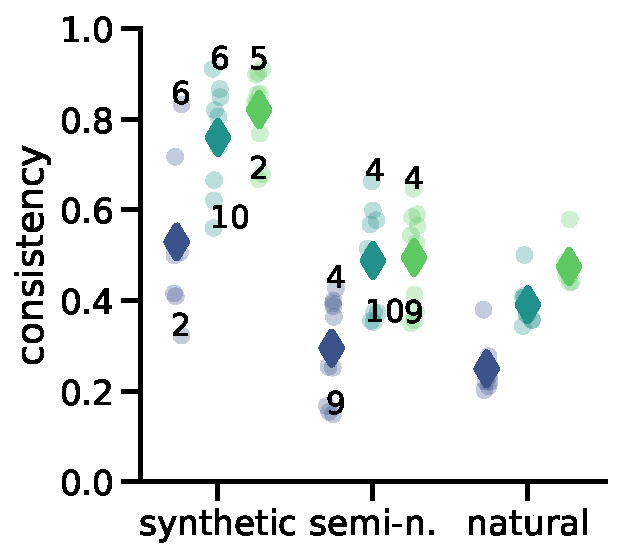
\includegraphics[width=\columnwidth]{figures/systematicity/s3.pdf}
        \caption{$\text{S}_1 \rightarrow \text{S}_3$}
        \label{fig:systematicity_sconj_s3}
    \end{subfigure}
    \begin{subfigure}[b]{0.45\columnwidth}
        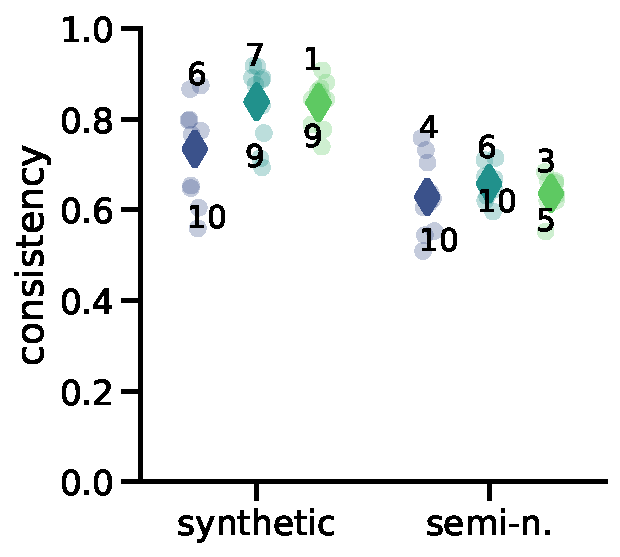
\includegraphics[width=\columnwidth]{figures/systematicity/np.pdf}
        \caption{$\text{NP} \rightarrow \text{NP}^\prime$}
        \label{fig:systematicity_snpvp_np}
    \end{subfigure}
    \begin{subfigure}[b]{0.49\columnwidth}
        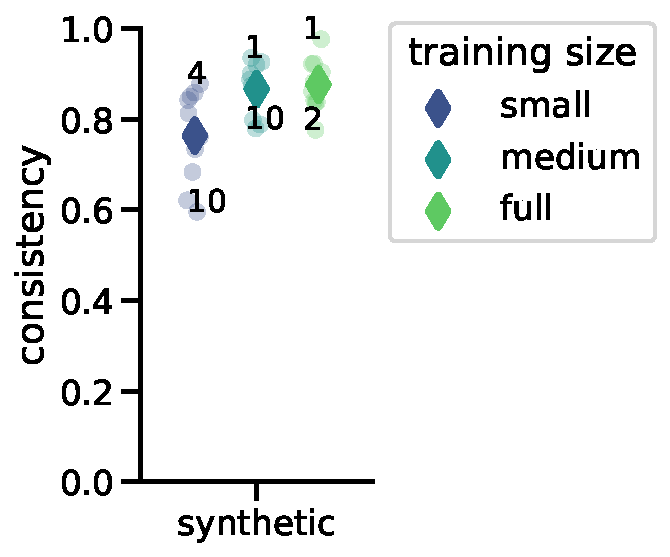
\includegraphics[width=\columnwidth]{figures/systematicity/vp.pdf}
        \caption{$\text{VP} \rightarrow \text{VP}^\prime$\hspace{8mm}}
        \label{fig:systematicity_snpvp_vp}
    \end{subfigure}
    \caption{Systematicity results for setup \texttt{\small S\;$\rightarrow$\;S\;CONJ\;S} (a and b) and \texttt{\small S\;$\rightarrow$\;NP\;VP} (c and d).
    Consistency scores are shown per evaluation data type ($x$-axis) and training dataset size (colours).
    Data points represent templates ($\circ$) and means over templates ($\diamond$).}
    \label{fig:systematicity}
\vspace{-0.3cm}
\end{figure*}


To evaluate our trained models, we adopt \textsc{Flores-101} \citep{goyal2021flores}, which contains 3001 sentences from Wikinews, Wikijunior and WikiVoyage, translated by professional translators, split across three subsets.
We train the models until convergence on the `dev' set.
Afterwards, we compute SacreBLEU scores on the `devtest' set \citep{post2018call}, using beam search (beam size = 5), yielding scores of $20.6\!\pm\!.4$, $24.4\!\pm\!.3$ and $25.8\!\pm\!.1$ for the small, medium and full datasets, respectively.\footnote{All training details are listed in Appendix~\ref{app:reproducibility}.}

\begin{figure}[t]\small
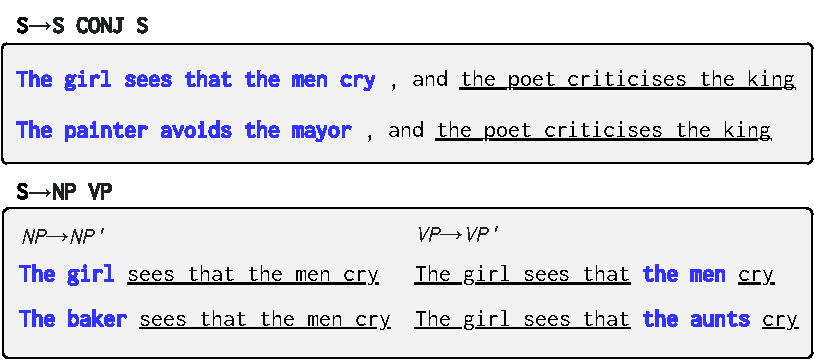
\includegraphics[width=\columnwidth]{figures/systematicity.pdf}
\caption{Illustration of the systematicity experiments \texttt{S\;$\rightarrow$\;S\;CONJ\;S} ($\text{S}_1$\;$\rightarrow$\;$\text{S}_3$ is shown) and \texttt{S\;$\rightarrow$\;NP\;VP} (both versions are shown).
Each experiment involves extracting translations before and after the replacement of the blue part, and then comparing the translation of the underlined words.}
\label{fig:systematicity_explanation}
\vspace{-0.3cm}
\end{figure}
